\special{! TeXDict begin /landplus90{true}store end }

\documentclass[xga]{xdvislides}
\usepackage[landscape]{geometry}
\usepackage{graphics}
\usepackage{graphicx}
\usepackage{colordvi}
\usepackage{tabularx}
\usepackage{multirow}

\newcommand{\smallish}{\fontsize{16}{16}\selectfont}

\begin{document}
\setfontphv

%% Headers and footers
\lhead{\slidetitle}                               % default:\lhead{\slidetitle}
\chead{CS615 - Aspects of System Administration}% default:\chead{\relax}
\rhead{Slide \thepage}                       % default:\rhead{\sectiontitle}
\lfoot{\Gray{Ethics and Social Responsibility}}% default:\lfoot{\slideauthor}
\cfoot{\relax}                               % default:\cfoot{\relax}
\rfoot{\Gray{\today}}

\vspace*{\fill}
\begin{center}
	\Hugesize
		CS615 - Aspects of System Administration\\ [1em]
		Ethics and Social Responsibility\\ [1em]
	\hspace*{5mm}\blueline\\ [1em]
	\Normalsize
		Department of Computer Science\\
		Stevens Institute of Technology\\
		Jan Schaumann\\
		\verb+jschauma@stevens.edu+\\
		\verb+https://www.cs.stevens.edu/~jschauma/615/+
\end{center}
\vspace*{\fill}

\subsection{Human $<->$ Computer Systems}
\vspace*{\fill}
\Huge
\begin{center}
Computering, at its heart, is a people problem. \\
\vspace{.5in}
System Administration, Software Engineering,
Information Security, etc. are all {\em social}
activities.
%activities influenced by and most effective when you
%consider the human at the keyboard.
\end{center}
\Normalsize
\vspace*{\fill}

\subsection{sudo(8)}
\vspace*{\fill}
\begin{verbatim}
We trust you have received the usual lecture from the local System
Administrator. It usually boils down to these three things:
#1) Respect the privacy of others.
#2) Think before you type.
#3) With great power comes great responsibility.
\end{verbatim}
\vspace*{\fill}

\subsection{The Job of a System Administrator}
What {\bf exactly} does a {\em System Administrator} do?
\begin{itemize}
	\item no precise job description
	\item often learned by experience
	\item ``makes things run''
	\item work behind the scenes
	\item often known as Operator, Network Administrator, System Programmer, System
		Manager, Service Engineer, Site Reliability Engineer etc.
\end{itemize}
\vfill
system administrator n.: \\
{\em one who, as a primary job function,
	manages computer and network systems on behalf of another, such as an
	employer or client.}

\subsection{Learning System Administration}
System Administration is a profession with no fixed career path.

\begin{itemize}
	\item few degree granting programs
	\item heavy reliance on practical experience
	\item specializations in many different areas possible
	\item breadth of expertise as necessary as depth in some areas
	\item background knowledge and requirements vary
\end{itemize}

\subsection{Wanted: Human Anatomy Engineer}
Required Skills and Experience:

\begin{itemize}
	\item 3+ years of poking humans with sharp objects
	\item must have previously diagnosed a fever
	\item MD preferred, or equivalent work experience
	\item experience performing brain surgery a plus
\end{itemize}

\subsection{Codes of Ethics}
\vspace*{\fill}
\begin{center}
	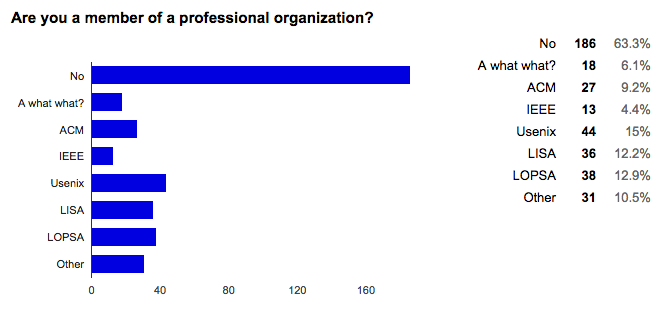
\includegraphics[scale=1.0]{pics/are-you-a-member.eps}
\end{center}
\vspace*{\fill}

\subsection{Codes of Ethics}
\vspace*{\fill}
\begin{center}
	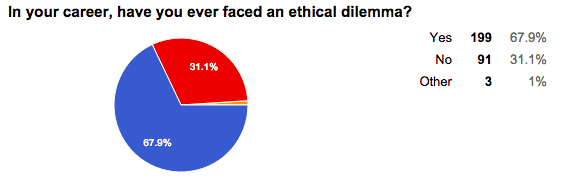
\includegraphics[scale=1.0]{pics/have-you-ever-faced-an-ethical-dilemma.eps}
\end{center}
\vspace*{\fill}

\subsection{Examples}
\begin{itemize}
	\item "I have teaching staff demanding access to students home directories."
	\item "Managers have asked me to spy on employees."
	\item "Snooping on specific employee's e-mail."
	\item "Faculty member child porn collection."
	\item "have been asked to lie to my direct reports (and candidates) about the future of the company"
	\item "have been told to not report various outages/loss of data situations to customers"
	\item "This is a daily thing."
\end{itemize}

\subsection{Legal != Ethical}
\vspace*{\fill}
\begin{center}
	
\includegraphics[scale=0.6]{pics/line.eps}
\end{center}
\vspace*{\fill}

\subsection{Legal != Ethical}
\vspace*{\fill}
\begin{center}
	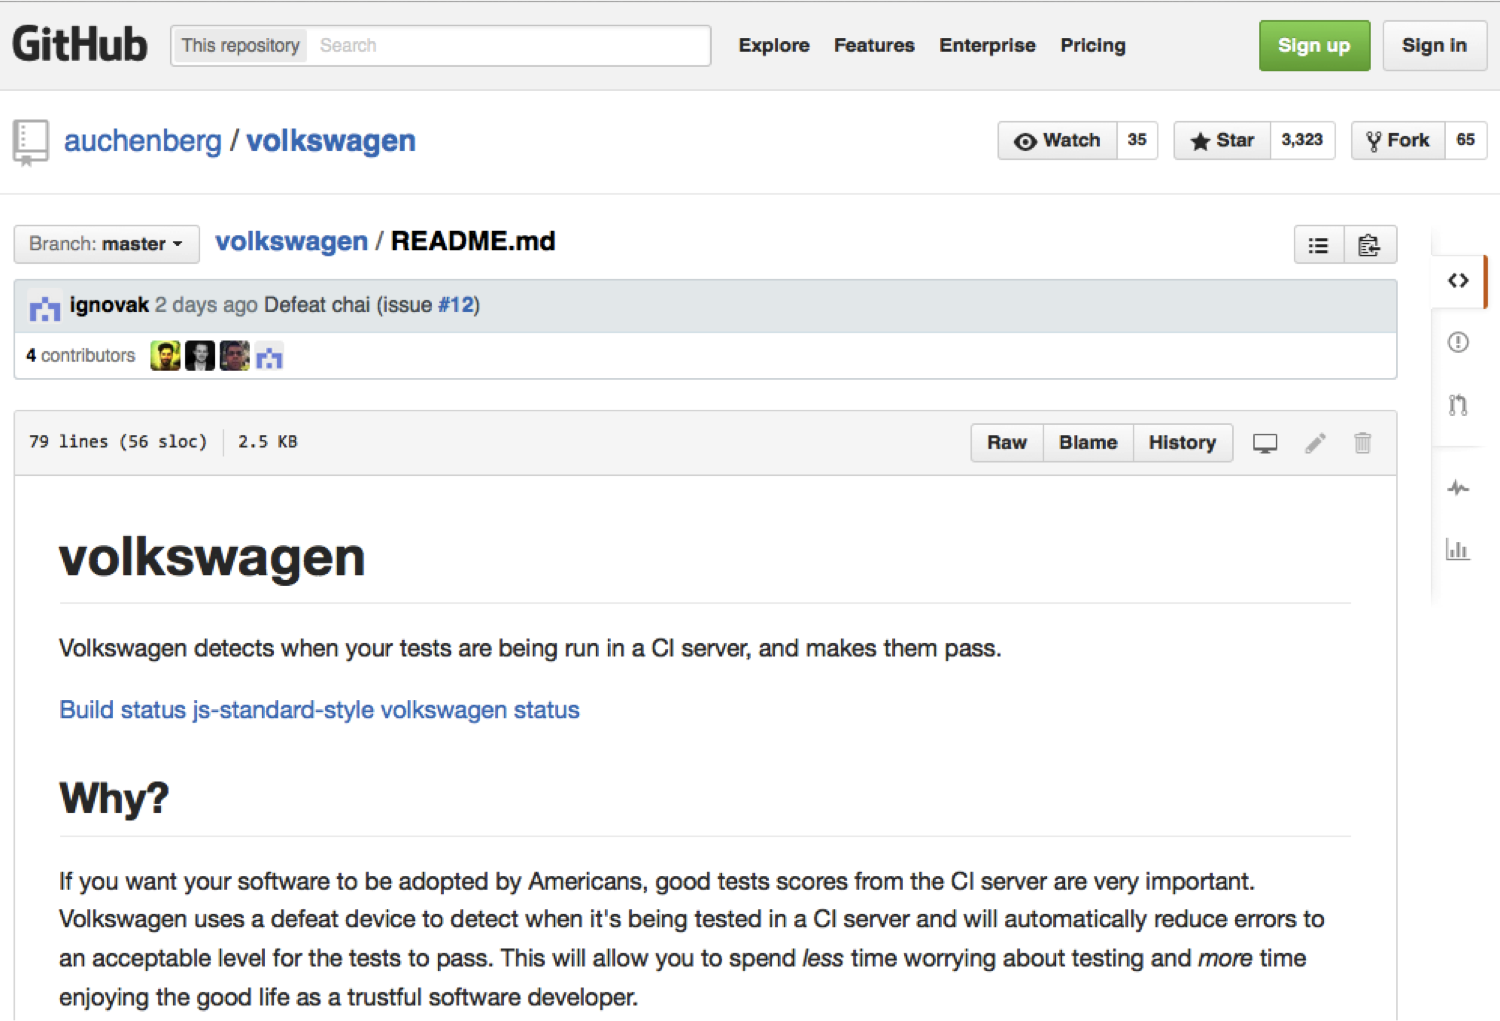
\includegraphics[scale=0.7]{pics/vw.eps}
\end{center}
\vspace*{\fill}

\subsection{Legal != Ethical}
\vspace*{\fill}
\begin{center}
	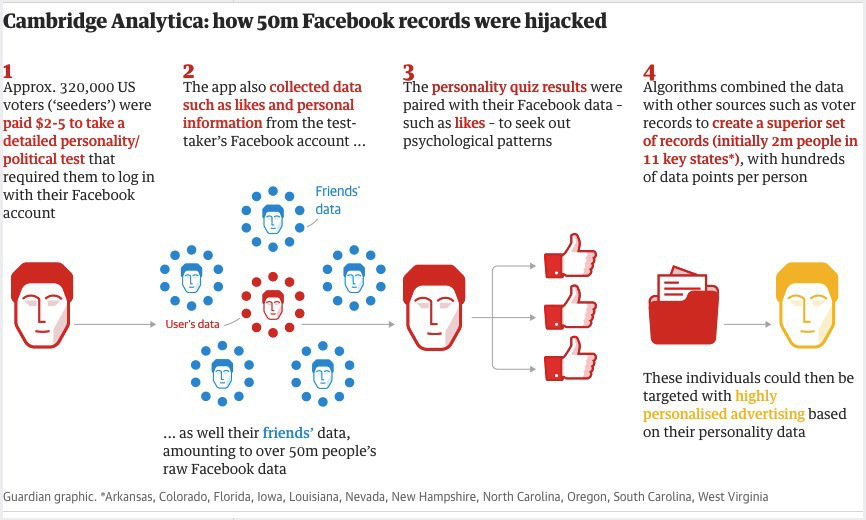
\includegraphics[scale=0.6]{pics/cambridge-analytica.eps} \\

	\small
	{\tt https://is.gd/IxFCRr}
	\Normalsize
\end{center}
\vspace*{\fill}



\subsection{Making the World A Better Place}
\vspace*{\fill}
\begin{center}
	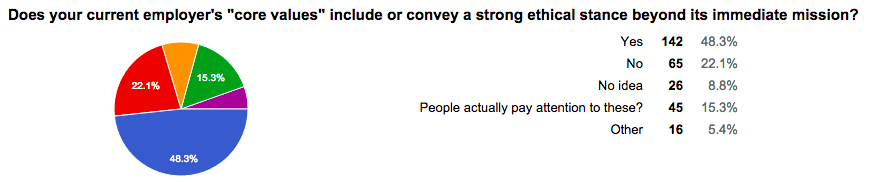
\includegraphics[scale=0.8]{pics/corporate-values.eps}
\end{center}
\vspace*{\fill}

\subsection{Making the World A Better Place}
\vspace*{\fill}
\begin{center}
	
\includegraphics[scale=1.0]{pics/silicon-valley.eps}
\end{center}
\vspace*{\fill}

\subsection{Making the World A Better Place}
Silicon Valley "Make The World A Better Place"
Business Plan:

\vspace*{\fill}
\begin{enumerate}
	\item offer some free service
	\item ???
	\item Profit!
\end{enumerate}
\vspace*{\fill}

\subsection{Making the World A Better Place}
Silicon Valley "Make The World A Better Place"
Business Plan:

\vspace*{\fill}
\begin{enumerate}
	\item offer some free service
	\item collect data, sell ads
	\item Profit!
\end{enumerate}
\vspace*{\fill}

\subsection{Codes of Ethics}
\Huge
\vspace*{\fill}
\begin{center}
	{\em Primum non nocere.}
\end{center}
\vspace*{\fill}
\Normalsize

\subsection{Codes of Ethics}
\vspace*{\fill}
\begin{center}
	
\includegraphics[scale=0.75]{pics/dont-be-a-dick.eps}
\end{center}
\vspace*{\fill}

\subsection{ACM Code of Ethics}
\Huge
\vspace*{\fill}
\begin{center}
1.1 Contribute to society and human well-being.
\end{center}
\vspace*{\fill}
\Normalsize

\subsection{(ISC)2 Code of Ethics}
\Huge
\vspace*{\fill}
\begin{center}
Protect society, the common good, necessary public
trust and confidence, and the infrastructure.
\end{center}
\vspace*{\fill}
\Normalsize

\subsection{IEEE Code of Ethics}
\Huge
\vspace*{\fill}
\begin{center}
to accept responsibility in making decisions
consistent with the safety, health, and welfare of the
public
\end{center}
\vspace*{\fill}
\Normalsize

\subsection{ACS Code of Ethics}
\Huge
\vspace*{\fill}
\begin{center}

{\bf The Primacy of the Public} \\
You will place the interests of the public
above those of personal, business or sectional
interests.

\end{center}
\vspace*{\fill}
\Normalsize

\subsection{A Code of Ethics in Internet Operations}
\Huge
\vspace*{\fill}
\begin{center}

We are stewards of our users' data. \\

We are obligated to act in the public interest.

\end{center}
\vspace*{\fill}
\Normalsize

\subsection{Ethics}
The LISA Code of Ethics:
\\

\newcolumntype{S}{>{\centering\arraybackslash} m{.4\linewidth} }
\begin{tabular}{ p{10cm} S }
\begin{itemize}
	\item Professionalism
	\item Personal Integrity
	\item Privacy
	\item Laws and Policies
	\item System Integrity
	\item Education
	\item Social Responsibility
	\item Ethical Responsibility
\end{itemize}
& \multirow{20}{*}{
\includegraphics[scale=1.3]{pics/angel.eps}} \\
\end{tabular}

\subsection{LISA Code of Ethics}
Professionalism and Personal Integrity:

\begin{itemize}
	\item maintain professional conduct; don't let
personal feelings or beliefs interfere
\end{itemize}

\subsection{LISA Code of Ethics}
Professionalism and Personal Integrity:

\begin{itemize}
	\item maintain professional conduct; don't let
personal feelings or beliefs interfere
	\item know your competence, know when to seek help
\end{itemize}

\subsection{LISA Code of Ethics}
Professionalism and Personal Integrity:

\begin{itemize}
	\item maintain professional conduct; don't let
personal feelings or beliefs interfere
	\item know your competence, know when to seek help
	\item disclose and recuse yourself under conflicts of interest
\end{itemize}

\subsection{LISA Code of Ethics}
Professionalism and Personal Integrity:

\begin{itemize}
	\item maintain professional conduct; don't let
personal feelings or beliefs interfere
	\item know your competence, know when to seek help
	\item disclose and recuse yourself under conflicts of interest
	\item own your mistakes
\end{itemize}

\subsection{LISA Code of Ethics}
Professionalism and Personal Integrity:

\begin{itemize}
	\item maintain professional conduct; don't let
personal feelings or beliefs interfere
	\item know your competence, know when to seek help
	\item disclose and recuse yourself under conflicts of interest
	\item own your mistakes
\end{itemize}
\vspace{.5in}
Lead by example.

\subsection{LISA Code of Ethics}
Privacy:
\begin{itemize}
	\item only access private information when necessary
\end{itemize}

\subsection{LISA Code of Ethics}
Privacy:
\begin{itemize}
	\item only access private information when necessary
	\item protect confidentiality of accidentally learned information
\end{itemize}

\subsection{LISA Code of Ethics}
Privacy:
\begin{itemize}
	\item only access private information when necessary
	\item protect confidentiality of accidentally learned information
	\item work in teams/pairs
\end{itemize}

\subsection{LISA Code of Ethics}
Privacy:
\begin{itemize}
	\item only access private information when necessary
	\item protect confidentiality of accidentally learned information
	\item work in teams/pairs
	\item delete, encrypt, anonymize
\end{itemize}

\subsection{LISA Code of Ethics}
Privacy:
\begin{itemize}
	\item only access private information when necessary
	\item protect confidentiality of accidentally learned information
	\item work in teams/pairs
	\item delete, encrypt, anonymize
	\item even better: do not collect the information to begin with
\end{itemize}

\subsection{LISA Code of Ethics}
Privacy:
\begin{itemize}
	\item only access private information when necessary
	\item protect confidentiality of accidentally learned information
	\item work in teams/pairs
	\item delete, encrypt, anonymize
	\item even better: do not collect the information to begin with
\end{itemize}
\vspace{.5in}
Data is a liability.

\subsection{Understand the OSI Stack}
\vspace*{\fill}
\begin{center}
	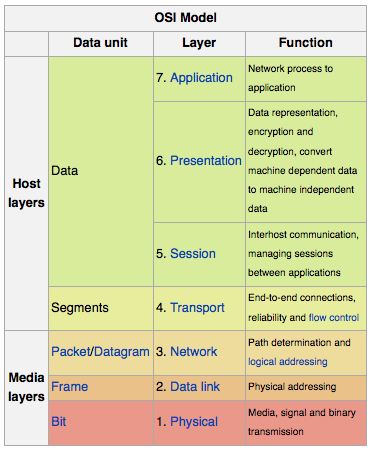
\includegraphics[scale=0.65]{pics/osi.eps}
\end{center}
\vspace*{\fill}

\subsection{LISA Code of Ethics}
Laws and Policies:
\begin{itemize}
	\item educate yourself and others on relevant laws, regulations, policies
\end{itemize}

\subsection{LISA Code of Ethics}
Laws and Policies:
\begin{itemize}
	\item educate yourself and others on relevant laws, regulations, policies
	\item (work to) elect informed representatives
\end{itemize}

\subsection{LISA Code of Ethics}
Laws and Policies:
\begin{itemize}
	\item educate yourself and others on relevant laws, regulations, policies
	\item (work to) elect informed representatives
	\item participate in design and architecture of e.g. technical standards
\end{itemize}

\subsection{LISA Code of Ethics}
Laws and Policies:
\begin{itemize}
	\item educate yourself and others on relevant laws, regulations, policies
	\item (work to) elect informed representatives
	\item participate in design and architecture of e.g. technical standards
	\item understand the difference between {\em
legal} and {\em ethical}; between the letter of a law
and the spirit or objective
\end{itemize}

\subsection{LISA Code of Ethics}
Laws and Policies:
\begin{itemize}
	\item educate yourself and others on relevant laws, regulations, policies
	\item (work to) elect informed representatives
	\item participate in design and architecture of e.g. technical standards
	\item understand the difference between {\em
legal} and {\em ethical}; between the letter of a law
and the spirit or objective
\end{itemize}
\vspace{.5in}
All politics is local.

\subsection{LISA Code of Ethics}
Communication:
\begin{itemize}
	\item communicate clearly, openly with your users, management, colleagues
\end{itemize}

\subsection{LISA Code of Ethics}
Communication:
\begin{itemize}
	\item communicate clearly, openly with your users, management, colleagues
	\item listen to the needs of others
\end{itemize}

\subsection{LISA Code of Ethics}
Communication:
\begin{itemize}
	\item communicate clearly, openly with your users, management, colleagues
	\item listen to the needs of others
	\item other people are also people
\end{itemize}

\subsection{LISA Code of Ethics}
Communication:
\begin{itemize}
	\item communicate clearly, openly with your users, management, colleagues
	\item listen to the needs of others
	\item other people are also people
	\item document your policies with reason and rationale
\end{itemize}

\subsection{LISA Code of Ethics}
Communication:
\begin{itemize}
	\item communicate clearly, openly with your users, management, colleagues
	\item listen to the needs of others
	\item other people are also people
	\item document your policies with reason and rationale
	\item let people see how you make decisions,
		how you prioritize things, how your team works
\end{itemize}


\subsection{LISA Code of Ethics}
Communication:
\begin{itemize}
	\item communicate clearly, openly with your users, management, colleagues
	\item listen to the needs of others
	\item other people are also people
	\item document your policies with reason and rationale
	\item let people see how you make decisions,
		how you prioritize things, how your team works
\end{itemize}
\vspace{.5in}
``Sunlight is the Best Disinfectant''

\subsection{LISA Code of Ethics}
Education and Community:
\begin{itemize}
	\item continously educate yourself, enhance your technical knowledge
\end{itemize}

\subsection{LISA Code of Ethics}
Education and Community:
\begin{itemize}
	\item continously educate yourself, enhance your technical knowledge
	\item share your knowledge, teach others
\end{itemize}

\subsection{LISA Code of Ethics}
Education and Community:
\begin{itemize}
	\item continously educate yourself, enhance your technical knowledge
	\item share your knowledge, teach others
	\item attending conferences is not optional
\end{itemize}

\subsection{LISA Code of Ethics}
Education and Community:
\begin{itemize}
	\item continously educate yourself, enhance your technical knowledge
	\item share your knowledge, teach others
	\item attending conferences is not optional
	\item eventually, neither is speaking at conferences
\end{itemize}

\subsection{LISA Code of Ethics}
Education and Community:
\begin{itemize}
	\item continously educate yourself, enhance your technical knowledge
	\item share your knowledge, teach others
	\item attending conferences is not optional
	\item eventually, neither is speaking at conferences
	\item publish your results, research
\end{itemize}

\subsection{LISA Code of Ethics}
Education and Community:
\begin{itemize}
	\item continously educate yourself, enhance your technical knowledge
	\item share your knowledge, teach others
	\item attending conferences is not optional
	\item eventually, neither is speaking at conferences
	\item publish your results, research
	\item build ties with peers at other organizations
\end{itemize}

\subsection{LISA Code of Ethics}
Education and Community:
\begin{itemize}
	\item continously educate yourself, enhance your technical knowledge
	\item share your knowledge, teach others
	\item attending conferences is not optional
	\item eventually, neither is speaking at conferences
	\item publish your results, research
	\item build ties with peers at other organizations
	\item partake in Open Source, meetups, mailing lists, community events
\end{itemize}

\subsection{LISA Code of Ethics}
Education and Community:
\begin{itemize}
	\item continously educate yourself, enhance your technical knowledge
	\item share your knowledge, teach others
	\item attending conferences is not optional
	\item eventually, neither is speaking at conferences
	\item publish your results, research
	\item build ties with peers at other organizations
	\item partake in Open Source, meetups, mailing lists, community events
\end{itemize}
\vspace{.5in}
You are shaped by the community and culture you choose. \\
Choose wisely.  Seek diversity.

\subsection{SysAdmin realities}
\begin{itemize}
	\item you are in a {\em privileged} position
\end{itemize}

\subsection{SysAdmin realities}
\begin{itemize}
	\item you are in a {\em privileged} position
	\item you {\em are} a target
\end{itemize}

\subsection{SysAdmin realities}
\begin{center}
	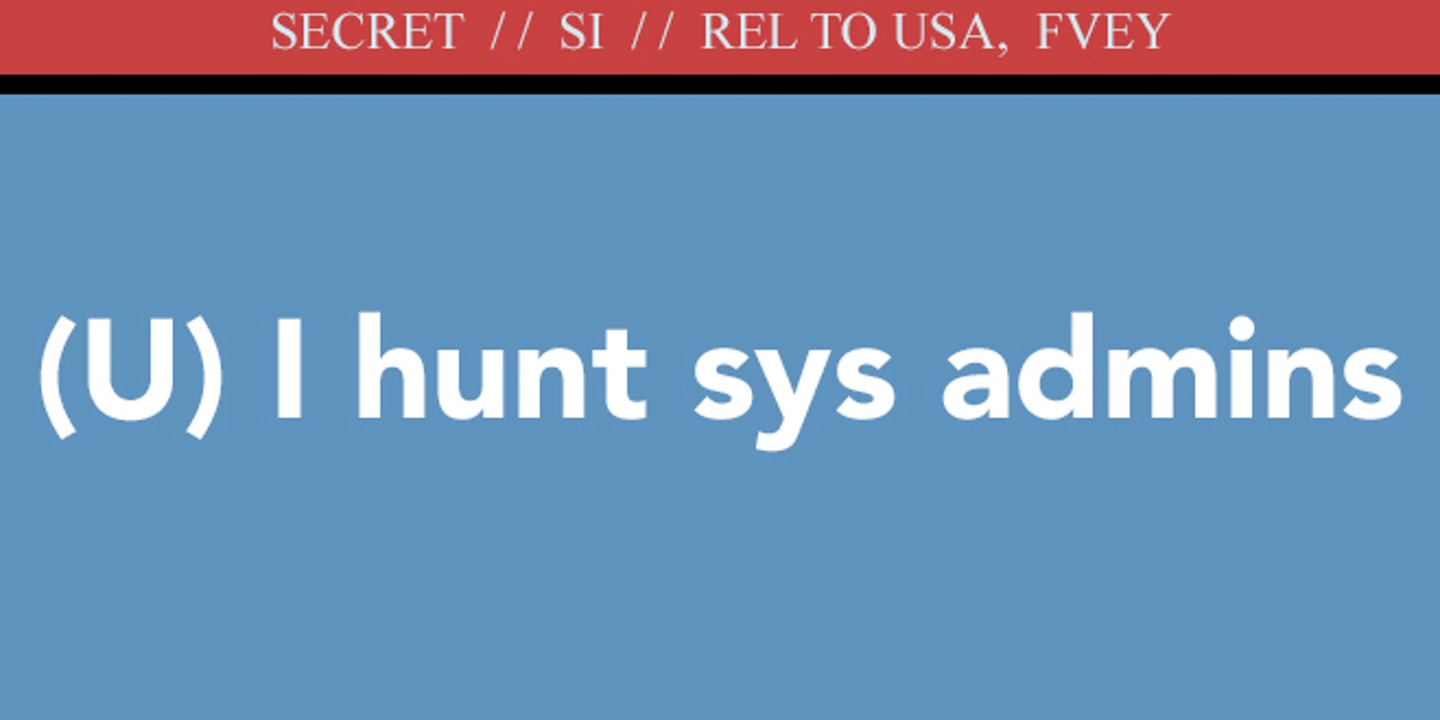
\includegraphics[scale=0.4]{pics/I-hunt-sys-admins.eps} \\
	\small
	{\tt https://is.gd/YURgRn}\hspace{.5in}{\tt https://is.gd/u8ni1B}
	\Normalsize
\end{center}

\subsection{SysAdmin realities}
\begin{itemize}
	\item you are in a {\em privileged} position
	\item you {\em are} a target
	\item you are {\em obligated} to act in your users' interest
\end{itemize}

\subsection{SysAdmin realities}
\begin{itemize}
	\item you are in a {\em privileged} position
	\item you {\em are} a target
	\item you are {\em obligated} to act in your users' interest
	\item you {\em will} face tough choices
\end{itemize}

\subsection{SysAdmin realities}
\begin{itemize}
	\item you are in a {\em privileged} position
	\item you {\em are} a target
	\item you are {\em obligated} to act in your users' interest
	\item you {\em will} face tough choices
	\item there is {\em no rulebook} to help you decide
\end{itemize}

\subsection{SysAdmin realities}
\begin{itemize}
	\item you are in a {\em privileged} position
	\item you {\em are} a target
	\item you are {\em obligated} to act in your users' interest
	\item you {\em will} face tough choices
	\item there is {\em no rulebook} to help you decide
	\item the slippery slope is not always steep
\end{itemize}

\subsection{SysAdmin realities}
\begin{itemize}
	\item you are in a {\em privileged} position
	\item you {\em are} a target
	\item you are {\em obligated} to act in your users' interest
	\item you {\em will} face tough choices
	\item there is {\em no rulebook} to help you decide
	\item the slippery slope is not always steep
	\item you {\em can} make a difference
\end{itemize}

\subsection{Ethics: This stuff isn't easy!}
\vspace{.5in}
\begin{center}
       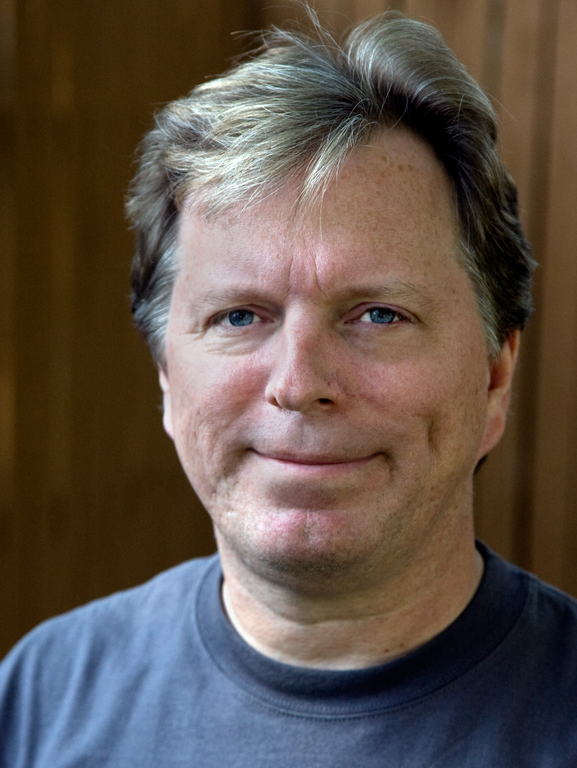
\includegraphics[scale=1.0]{pics/merlyn.eps} \\

	\small
	{\tt https://is.gd/mvHzIX}\hspace{.5in}{\tt https://is.gd/djUzAO}
	\Normalsize
\end{center}


\subsection{Ethics: This stuff isn't easy!}
\vspace{.5in}
\begin{center}
       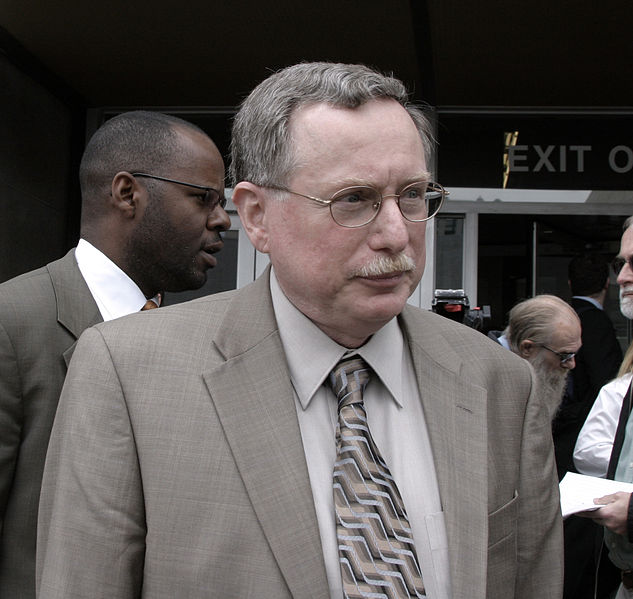
\includegraphics[scale=0.35]{pics/mark-klein.eps}
       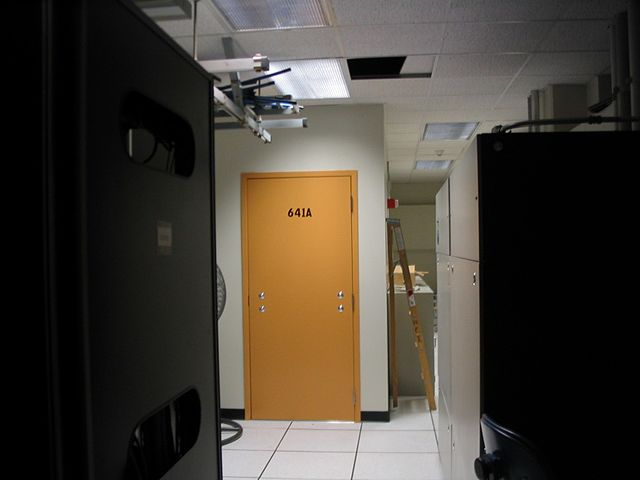
\includegraphics[scale=0.45]{pics/Room_641A.eps} \\

	\small
	{\tt https://en.wikipedia.org/wiki/Room\_641A}
	\Normalsize
\end{center}


\subsection{Ethics: This stuff isn't easy!}
\begin{center}
       
\includegraphics[scale=0.3]{pics/snowden.eps}
\end{center}

\subsection{Being good stewards}
\Huge
\vspace*{\fill}
\begin{center}

Speak up, ask questions. \\

\vspace{.5in}

{\em ``All that is necessary for the triumph of evil is
that good people do nothing.''}

\end{center}
\vspace*{\fill}
\Normalsize


\subsection{At the end of the day...}
\begin{center}
	
\includegraphics[scale=0.5]{pics/thumbsup-borat.eps}
\end{center}

\subsection{Reading}
\begin{itemize}
	\item \verb+https://www.usenix.org/lisa/system-administrators-code-ethics+
	\item \verb+http://www.acm.org/about/code-of-ethics+
	\item \verb+https://www.netmeister.org/blog/primum-non-nocere.html+
	\item \verb+https://www.netmeister.org/blog/all-is-not-lost.html+
	\item \verb+https://www.netmeister.org/blog/semper-ubi-sub-ubi.html+
	\item \verb+http://neveragain.tech/+
\end{itemize}

\subsection{Professional Organizations}
\begin{itemize}
	\item \verb+https://www.usenix.org/+ and \verb+https://www.usenix.org/lisa+
	\item \verb+http://www.lopsa.org/+
	\item \verb+http://www.acm.org/+
	\item \verb+https://www.internetsociety.org/+
	\item \verb+https://www.nanog.org/+
\end{itemize}

\end{document}
